\chapter{Limitations}
\label{sec:limitations}

Now we turn to discuss the design limitations of Trusted Capsules. In this
section we cover the limitations imposed by our design choices and the
limitations imposed by the specific choice of software and hardware. Moreover,
we take a gander at why Trusted Capsules remains a rather naive attempt at
solving the problem of retrofitting existing applications with security
extensions.

\subsection{Desgin Limitations}
\begin{enumerate}
    \item {\bf Inability to limit trust in optimistic state}: In the optimistic state, we
trust the normal world kernel, the app, and the user, to not leak capsule data
to unauthorized apps. Such trust may not be warranted even in a non-adversarial
setting. For example, an app might create temporary copies of the files it has
opened into a world-readable directory or the user might copy the data into the
system clipboard. While we may use techniques such as information flow control
to detect such data leaks, doing so would prohibitively impact performance.

    \item {\bf Lack of app semantics}: Since we interpose only on the {\tt open()} and
    {\tt close()} syscalls to execute policies, a policy may not reason about {\em
        why} an app is opening a file. For example, when a user opens a document in a
text editor, it may open the file multiple times to seek through the file in
parallel. Hence, while the capsule was opened just once from a user's
perspective, the policy would observe multiple capsule access attempts. Policies
that rely on access logs have to be aware of this disconnect.

    \item {\bf Abusive policies}: Although we run capsule policies in a sandbox, we do not
completely prevent all damages a malicious policy can inflict. It can, for
example, access a user's GPS data and send them to a server for the purpose of
tracking her whereabouts. To handle this limitation, we either need some
systematic way of vetting the data a policy sends to a remote server or prevent
it from sending device data altogether.
\end{enumerate}

%%%%%%%%%%%%%%%%%%%%%%%%%%%%%%%%%%%%%%%%%%%%%%%%%%%%%%%%
\begin{figure}[t]
    \centering
    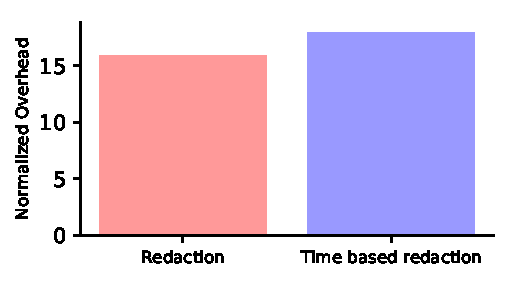
\includegraphics[width=8cm,height=4cm]{fig/policy_latencies.pdf}
    \caption{Normalized latency of servicing an \texttt{open} for different policies with respect to the latency to service a null-policy capsule open request. }
    \label{fig:policy_latency}
\end{figure}
%%%%%%%%%%%%%%%%%%%%%%%%%%%%%%%%%%%%%%%%%%%%%%%%%%%%%%%%


\subsection{Prototype Limitations:}
In this section we list the limitations that bound the current prototype from
realizing the fulll vision of the Trusted Capsule model of data protection.
Here we note some design and implementation limitations.

\begin{enumerate}
    \item FUSE can be used interpose on only the file I/O system calls that are
directed to a FUSE serviced mountpoint. This poses some challenges in making
Trusted Capsules work seamlessly with an unmodified application.\\There is no
way for the FUSE filesystem code to identify when a process that had been
issuing IO to the mountpoint dies. The implication of this fact for the
prototype is that there is no good and atomic way to delete the shadow file on
the termination of the process. The prototype handles this by setting up a
background process that monitors if the process that had accessed the mountpoint
has terminated.
    \item The stock configuration for the TrustZone memory partitions makes the
Secure World a very memory constrained environment. The memory that is available
in the secure world is only 10 MB, and that needs to host the Secure OS as well
as any trusted application code that must run in Trustzone. Linaro OP-TEE
recently included dynamic shared memory in their Secure OS, but to access those
features, one has to have a higher kernel version than what gets shipped with
the stock Debian OS rootfs image. Higher Linux kernel versions have known
problems with the HDMI drivers, which causes the Linux kernel to panic when a
monitor is plugged in.
    \item This limitation hits our prototype particularly badly. In the
current prototype, we send a copy of the entire file to TrustZone to decrypt.
Since there are severe restrictions on the amount of memory available in
TrustZone, we are unwittingly bounded on the maximum file size that can be
processed as a capsule.
    \item The implementation has a limitation that it
needs to create copies of the data buffers to process each part of the capsule.
This creates more memory pressure in an already resource constrained
environment. 
\end{enumerate}

